\documentclass{article}

\usepackage{graphicx}
\usepackage{amsmath}
\usepackage{xcolor}
\usepackage{stackengine}

\newcommand{\flecha}[2] {
    \!\!$\overset{\text{#1}}{\overset{\downarrow}{\text{#2}}}$\!\!
}

\usepackage{geometry}
 \geometry{
 a4paper,
 total={170mm,257mm},
 left=20mm,
 top=20mm,
 }

\graphicspath{{./Imagenes/}}

\begin{document}
\section*{Explicacion del algoritmo}

\subsection*{Idea inicial}
El objetivo del programa es el de poder identificar las palabras a espaciar en una única lectura del texto de entrada.
Para ello es necesario poder rastrear multiples palabras del diccionario al mismo tiempo.

Para lograr esto se guardan todas las palabras en un árbol general, cada nodo del árbol va a representar un posible
prefijo de una palabra del diccionario. Las aristas del árbol se etiquetan con un carácter del alfabeto, de modo que si
un nodo A con la palabra p esta conectado a otro nodo B mediante una arista con el carácter 'c', entonces la palabra
que contiene el nodo B es p+c.

Por ejemplo el árbol para el diccionario ["quien", "deposito", "dolar", "dolares", "es", "recibira"] es:

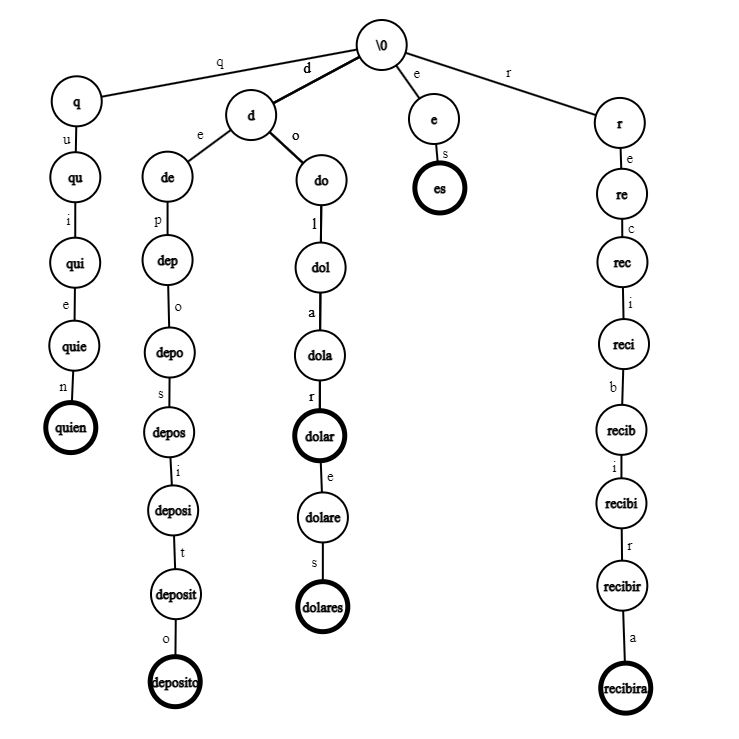
\includegraphics[scale=0.3]{trie1.png}

Los nodos a su vez tienen que indicar si el prefijo representa una palabra que esta en el diccionario, en el gráfico
eso queda representado por un circulo de un color mas fuerte.

Usando este árbol, se puede analizar el string como sigue. Se inicializan dos iteradores i,j al inicio de la palabra a analizar,
en cada paso se mueve el iterador j y se recorre el árbol en la arista correspondiente. Si en algún momento se llega a un nodo
con una palabra del diccionario se guarda la posicion actual en una variable k(esta variable se sobrescribe si se encuentra otra
palabra mas grande). Cuando se llega a un punto en el que no se puede seguir por el árbol, la palabra encontrada es el substring
[i:k]. Despues se avanza el iterador i hasta k+1(hasta i+1 en el caso en que no se encontro una palabra) y se vuelve a la raíz del 
arbol para continuar el analisis.

Asi para el diccionario de ejemplo, la palabra "dosdolares" se espacia de esta forma:

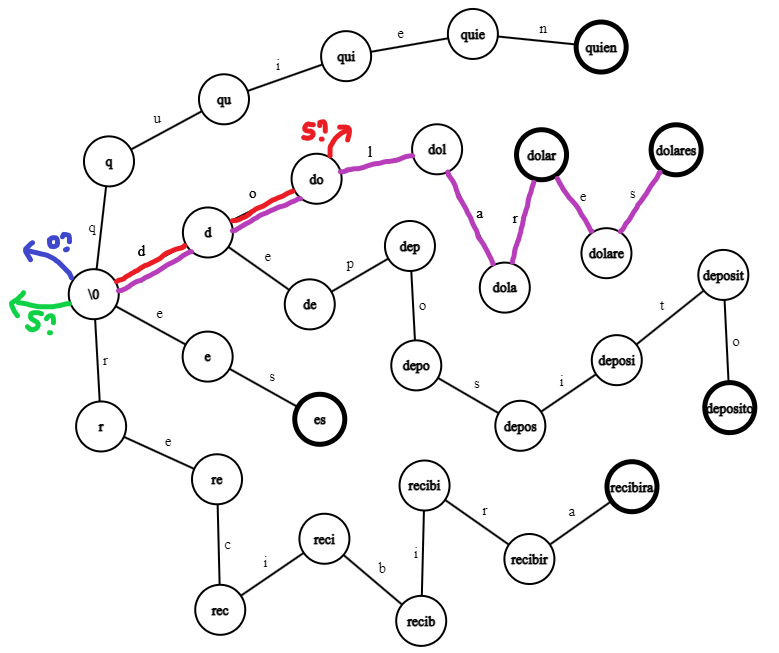
\includegraphics[scale=0.4]{ejemplo_trie1.png}

{\color{red} 1:} \flecha{i,j}{d}osdolares $\rightarrow$ \flecha{i}d\flecha{j}osdolares $\rightarrow$ \flecha{i}do\flecha{j}sdolares $\rightarrow$ {\color{red} \textbf X}

El nodo "do" no tiene una arista con el carácter 's', como no se puede seguir vuelvo a la raíz y avanzo i un lugar para adelante.

{\color{blue} 2:} d\flecha{i,j}osdolares $\rightarrow$ {\color{red} \textbf X}

La raíz no tiene una arista con el carácter 'o', como no se puede seguir, paso al carácter siguiente.

{\color{green} 3:} do\flecha{i,j}sdolares $\rightarrow$ {\color{red} \textbf X}

La raíz no tiene una arista con el carácter 's', como no se puede seguir, paso al carácter siguiente.

{\color{violet} 4:} dos\flecha{i,j}dolares $\rightarrow$ dos\flecha{i}d\flecha{j}olares $\rightarrow$ dos\flecha i do\flecha j lares
$\rightarrow$ dos\flecha i dol\flecha j ares $\rightarrow$ dos\flecha i dola\flecha j res

Se encontro la palabra "dolar", se marca con una flecha k

dos\flecha i dola\flecha k r\flecha j es $\rightarrow$ dos\flecha i dola\flecha k r e\flecha j s $\rightarrow$ {\color{red}\textbf{X}}

Se encontro la palabra "dolares", se marca con una flecha k:

dos\flecha i dolare\flecha k s $\rightarrow$ {\color{red}\textbf{X}}

No se puede seguir porque se termino de leer el string, la palabra mas large encontrada fue "dolares":

La salida final del programa es: "dolares"

Esta idea no es lo suficientemente optima ya que el indice j tiene que retroceder junto al indice i para analizar caracteres que
ya fueron revisados. Esto hace que en algunos casos el algoritmo realiza $n^2$ operaciones, donde $n$ es el largo del string. Es el caso
de la palabra "cinco" con el diccionario ["cincos","incos","ncos","cos","os","s"]

Para poder evitar esto, es necesario agregar información adicional en el árbol.

\subsection*{Optimización: transiciones de falla}

La idea de la optimización es que si no se puede seguir recorriendo el arbol desde un nodo B, en vez de volver a la raíz y recorrer desde ahi hasta un cierto nodo A,
se salte directamente del nodo B al nodo A. De esta manera se "reciclan" los caracteres que habia entre $i$ y $j$ en vez leerlos nuevamente.

Dado que es posible llegar desde el nodo raiz hasta el nodo A usando uno o mas de los caracteres finales de B. El prefijo que representa A es a su vez
un sufijo propio de B. Solo hace falta añadir una restriccion adicional, el sufijo propio no puede contener parte de una palabra aceptada(sino podria pasar que se acepten dos palabras que se solapan),
por eso tiene que ser un sufijo propio que no contenga parte de una palabra aceptada.

Así, se puede añadir a cada nodo del arbol que representa el prefijo X una arista que apunte a otro nodo del árbol que represente su 
sufijo propio más largo(transición de falla). 

Estas serian algunas de las transiciones de falla para el arbol de ejemplo. Las aristas en rojo marcan las transiciones de falla. Dado que pueden ser muchas,
los nodos que no tienen aristas rojas tienen su transición de falla apuntando a la raíz:

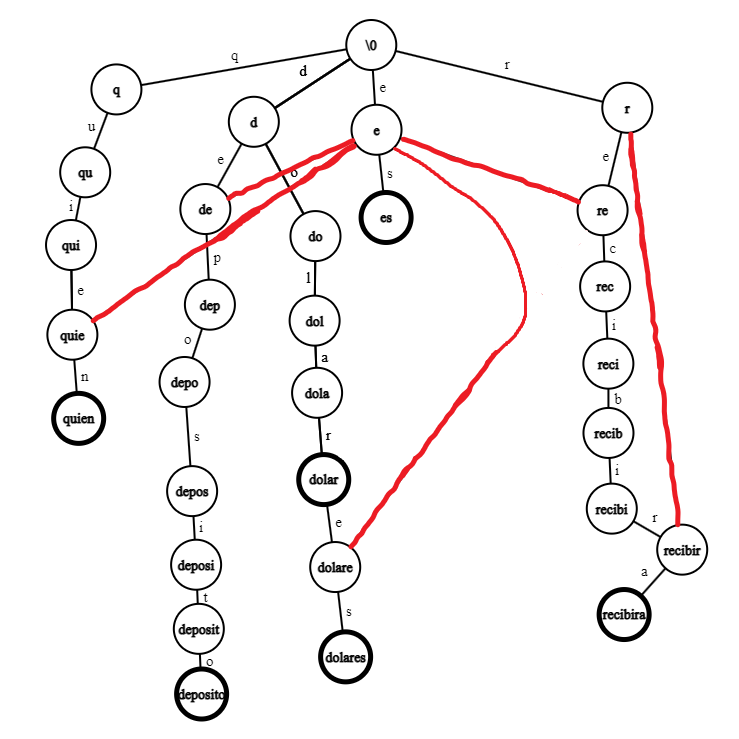
\includegraphics[scale=0.5]{Imagenes/trie1_transiciones_falla.png}


De esta forma, si en un cierto punto se quiere leer el carácter 'x' y el nodo actual no posee una arista con dicho carácter,
se sigue la transición de falla y se revisa si es posible seguir desde ahi con el carácter 'x', en caso contrario se sigue la transición de falla del nodo al que recién se llego y se repite el proceso.

Eventualmente las transiciones de falla terminan en la raíz, si se llega hasta la raíz y no es posible seguir con el caracter 'x', entonces se descarta el caracter y se sigue leyendo el string.

Con las transiciones de falla incluidas, el árbol ya puede usarse como si fuera un Autómata de Estado Finito(de hecho, asi es como se lo llama en el código).

Para el ejemplo de la palabra "dosdolares", con el diccionario ["dolar","dolares"] el espaciado se calcularia asi:

\begin{center}
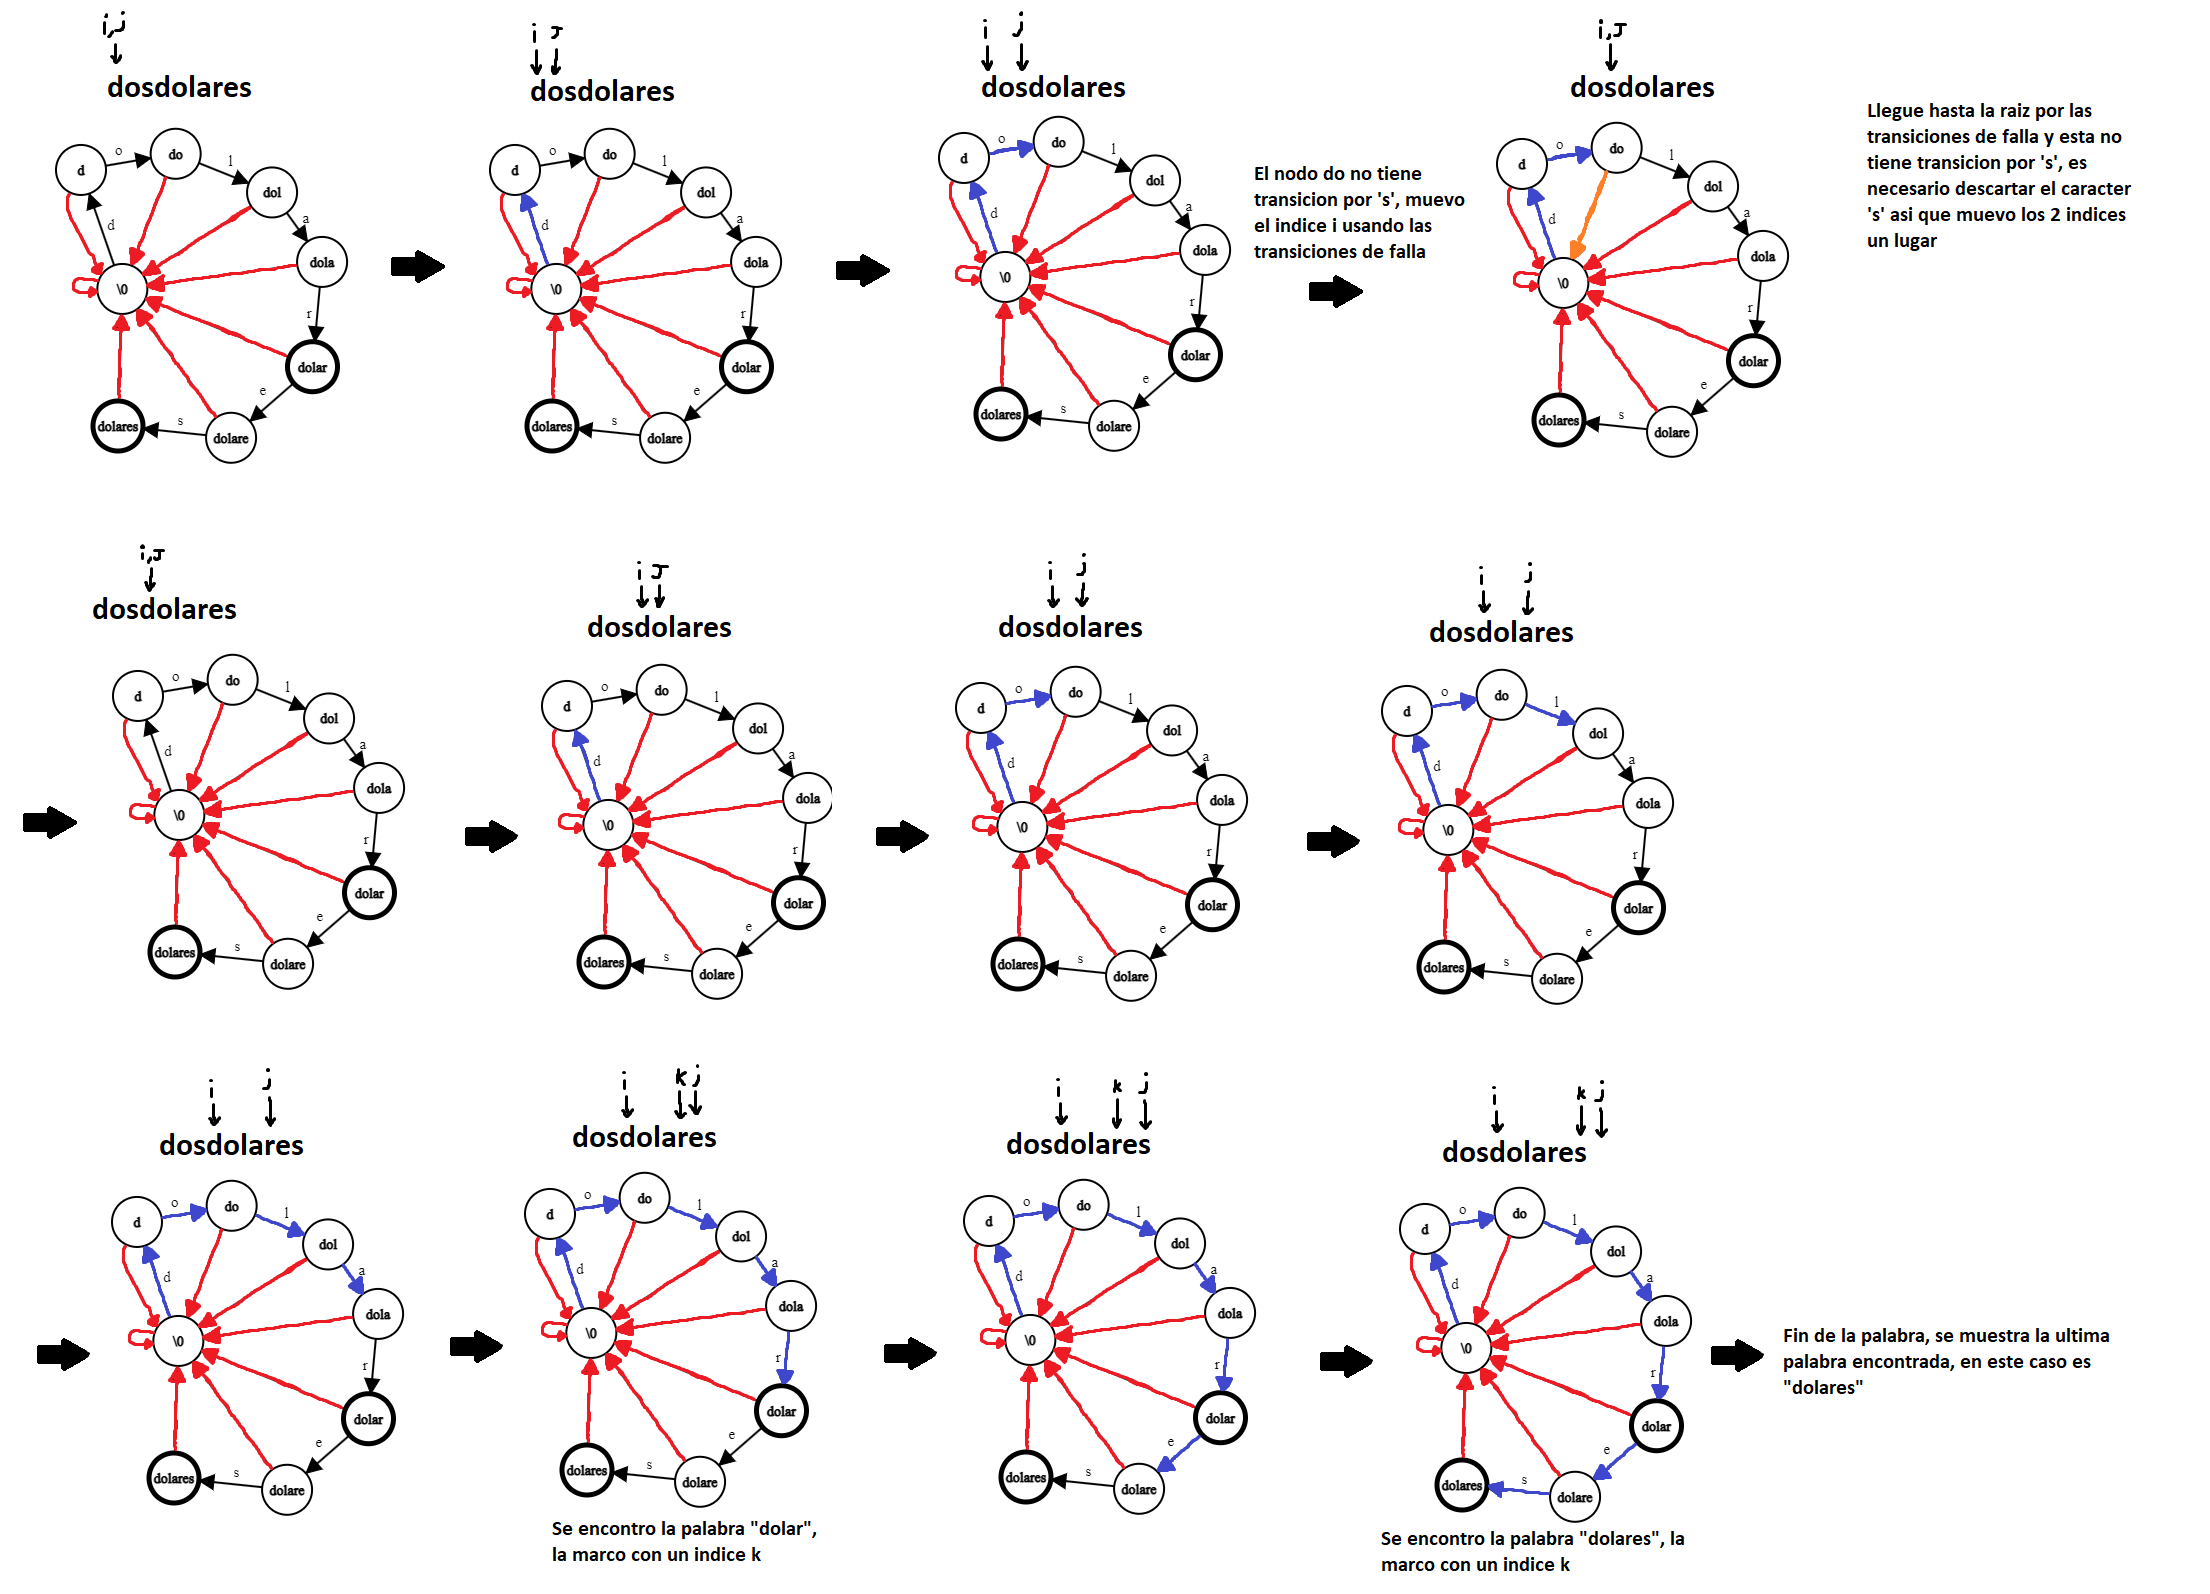
\includegraphics[scale=0.3]{Imagenes/automata_falla_ejemplo_dosdolares.png}
\end{center}

Suponiendo que el autómata ya esta construido, espaciar una palabra tiene una complejidad $O(n+z)$ donde $n$ es el largo de la palabra y $z$ es la suma de todos los largos de las palabras encontradas.
El n viene de que cada letra de la palabra es visitada una sola vez por los indices $i$ y $j$ que avanzan linealmente. El $z$ viene de que para mostrar una palabra encontrada hay que recorrerla de principio
a fin, por lo que en total mostrar todas las palabras cuesta $O(z)$.

\newpage

Sin embargo el algoritmo tiene errores, por ejemplo, para la palabra "dola" y el diccionario ["dolar","ol"] el algoritmo es como sigue:

\begin{center}
    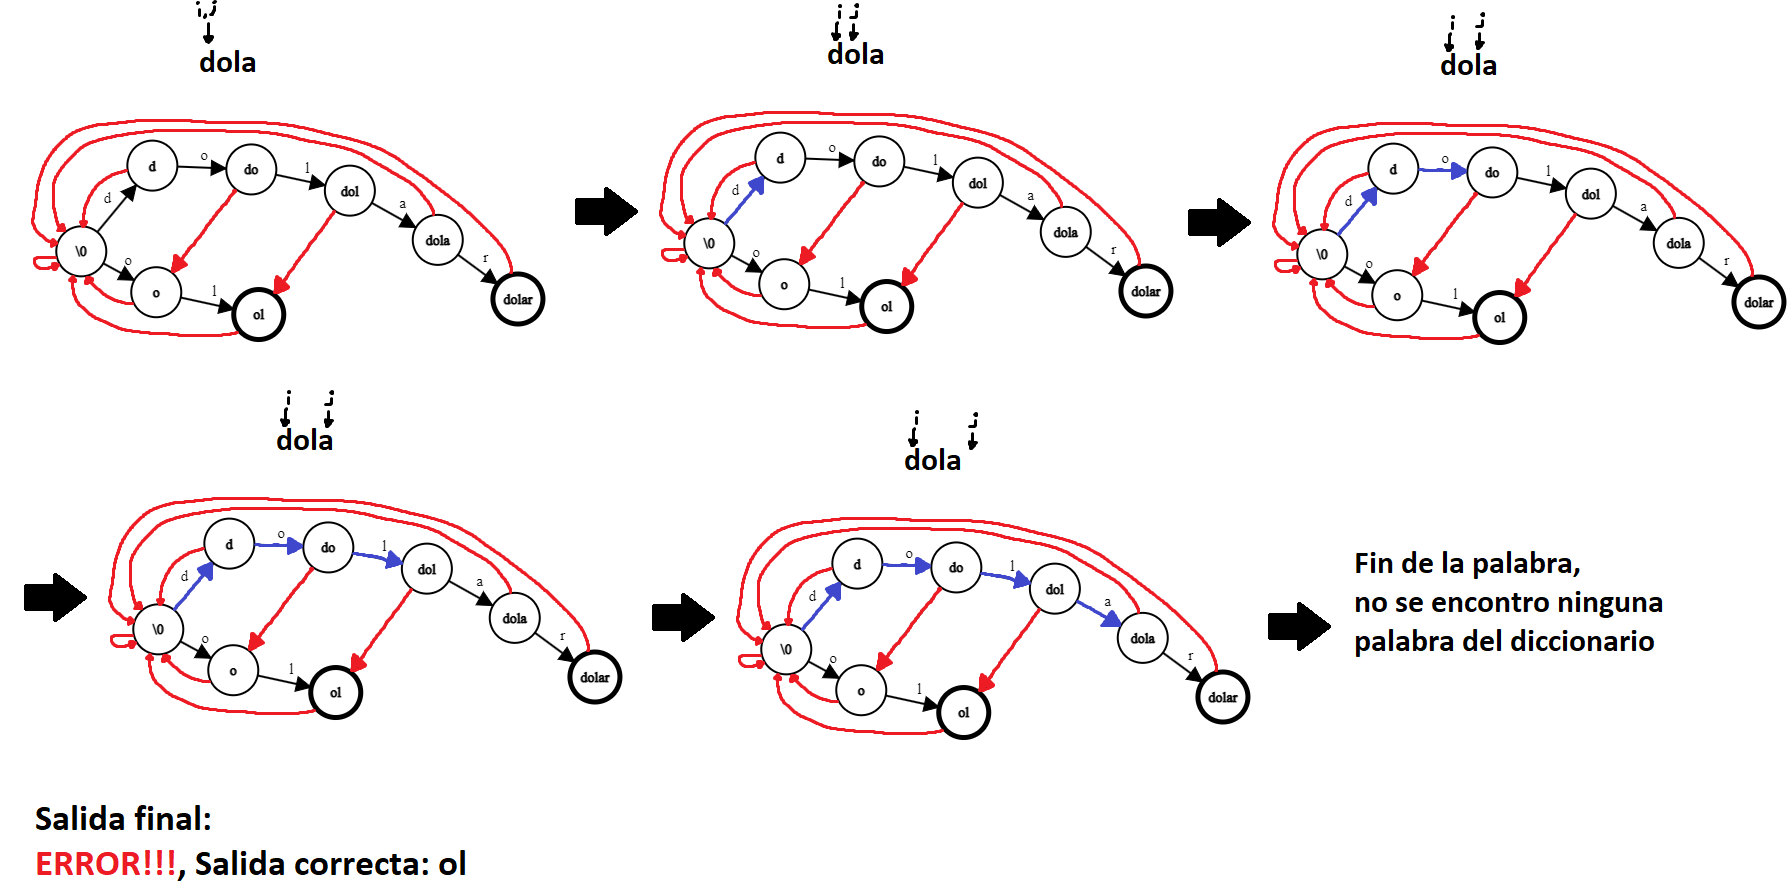
\includegraphics[scale=0.3]{Imagenes/automata_falla_ejemplo_dola.png}
\end{center}

\subsection*{Solución: transiciones de salida}

Un primer intento de solucionar este problema es que cuando se llega a un estado cualquiera, se empiezan a recorrer las transiciones de salida
hasta la raíz, si en el camino se encuentra un estado de aceptación entonces se registra de alguna manera que una palabra se encontró.
Como la distancia entre 2 estados de aceptación unidos por transiciones de falla puede ser bastante grande, esta opcion puede resultar ineficiente.

Para optimizar esta solución se pueden añadir nuevas transiciones al autómata, las \textbf{transiciones de salida}, que apunten a un nodo que representa al sufijo
propio mas grande que es a su vez una palabra del diccionario. Para el ejemplo anterior, la transición de salida del nodo con la palabra "dol" apuntaria al nodo con la palabra "ol" y
todos los nodos restantes quedan sin transición de salida.

De esta manera, cuando se llega a un nodo cualquiera, se recorren las transiciones de salida y se registran las palabras encontradas en el camino. Si bien el metodo es igual al anterior, este
es mas eficiente ya que solo visita los nodos de aceptación y se "saltea" los nodos que no son de aceptación.




\end{document}